%compile with xelatex --shell-escape ContextFreeConstrainedPathFindingInGraph.tex

% v2-acmtog-sample.tex, dated March 7 2012
% This is a sample file for ACM Transactions on Graphics
%
% Compilation using 'acmtog.cls' - version 1.2 (March 2012), Aptara Inc.
% (c) 2010 Association for Computing Machinery (ACM)
%
% Questions/Suggestions/Feedback should be addressed to => "acmtexsupport@aptaracorp.com".
% Users can also go through the FAQs available on the journal's submission webpage.
%
% Steps to compile: latex, bibtex, latex latex
%
% For tracking purposes => this is v1.2 - March 2012
\documentclass{sig-alternate} % V1.2

%\acmVolume{VV}
%\acmNumber{N}
%\acmYear{YYYY}
%\acmMonth{Month}
%\acmArticleNum{XXX}
%\acmdoi{10.1145/XXXXXXX.YYYYYYY}
\usepackage{graphicx}
\usepackage{caption}
\usepackage{subcaption}
\usepackage{gnuplottex}
\usepackage{tikz}
%\usepackage[T2A]{fontenc} 
%\usepackage[utf8]{inputenc}
\usepackage{graphicx}
%\usepackage{indentfirst}
\usepackage{hyperref}
\usepackage{textcomp}

\begin{document}

\newtheorem{mytheorem}{Theorem}
\newtheorem{lemma}{Lemma}

\makeatletter
\def\@copyrightspace{\relax}
\makeatother

\title{Generalized LL parsing for context-free constrained path search problem}

\sloppy

\numberofauthors{2}

\author{
\alignauthor
       Semyon Grigorev\\
       \affaddr{Saint Petersburg State University}\\
       \affaddr{7/9 Universitetskaya nab.}\\
       \affaddr{St. Petersburg, 199034 Russia}\\
       \email{semen.grigorev@jetbrains.com}
\alignauthor
       Anastasiya Ragozina\\
       \affaddr{Saint Petersburg State University}\\
       \affaddr{7/9 Universitetskaya nab.}\\
       \affaddr{St. Petersburg, 199034 Russia}\\
       \email{ragozina.anastasiya@gmail.com}
}

\maketitle

\begin{abstract}
Aaaabstract is very abstract.... 
word1 word2 word3 word4 word5 word6 word7 word8 word9 word10
word1 word2 word3 word4 word5 word6 word7 word8 word9 word10
word1 word2 word3 word4 word5 word6 word7 word8 word9 word10
word1 word2 word3 word4 word5 word6 word7 word8 word9 word10
word1 word2 word3 word4 word5 word6 word7 word8 word9 word10
word1 word2 word3 word4 word5 word6 word7 word8 word9 word10
word1 word2 word3 word4 word5 word6 word7 word8 word9 word10
word1 word2 word3 word4 word5 word6 word7 word8 word9 word10
word1 word2 word3 word4 word5 word6 word7 word8 word9 word10
word1 word2 word3 word4 word5 word6 word7 word8 word9 word10

\end{abstract}
!!!!!!!!НЕ ЗАБЫВАЙ, ЧТО ПОСЛЕ СУЩЕСТВИТЕЛЬОГО В ЕДИНСТВЕННОМ ЧИСЛЕ ГЛАГОЛЫ С ОКОНЧАНИЕМ S!!!
\section{Introduction}
Graph data model and graph data bases are very popular in many different areas such as bioinformatic, semantic web, social networks etc.
Extraction of paths satisfying specific constraints may be useful for graph structured data investigation and for relations between data items detection.
Path querying with constrains formulated in terms of formal grammars is a specific problem named formal language constrained path problem~\cite{FLCpathProblem} and research in this area is still actual~\cite{DirOfBigGraphAnalysis}.
!!!!!!!!!!!!!!!!!!!!!!!!!!!!!!!!!!!!!!!!!!!!
Information from different areas such as bioinformatic, semantic web, social networks can be represened in graph model. Moreover, there are data graph data bases. (?) One of the common graph problem is paths extraction from graph. Paths must satisfy specific constrains and the search must use a reasonable time. (?)     
!!!!!!!!!!!!!!!!!!!!!!!!!!!!!!!!!!!!!!!!!!!!
Classical parsing techniques can be used to solve formal language constrained path problem thus we can use ``graph parsing'' and it may be required not only in graph data base quering but also in other 
different areas: formal verification, and string-embedded language processing, for example. 

!!!!!!!!!!!!!!!!!!!!!!!!!!!!!!!!!!!!!!!!!!!!
Classical parsing techniques can be used to solve formal language constrained path problem. It means that such technique can be used on more common problem -- ``graph parsing''. Graph parsing may be required in graph data base quering, formal verification, string-embedded language processing and another areas where graph structured data. 
!!!!!!!!!!!!!!!!!!!!!!!!!!!!!!!!!!!!!!!!!!!!

The moste solution in DB area use such parsing algorithms as CYK or Earley.
In string-embedded languages analysis (RN)GLR is used.
It has better time complexity.
!!!!!!!!!!!!!!!!!!!!!!!!!!!!!!!!!!!!!!!!!!!!!!!
Parsing technique are used in DB previously. Usually this aproach use CYK or Earley algorithms. (WHAT PROBLEM and why string embedded lang?) нужны ли нам тут вообще встроенные языки и упоминания про них? ЕСЛИ НУЖНЫ, ТО ЛУЧШЕ ОБЪЯСНИТЬ ЗАЧЕМ, ЕСЛИ ВО ВВЕДЕНИИ ЭТО НЕВАЖНО, НО ВАЖНО ДАЛЬШЕ, ТО МОЖНО ОБ ЭТОМ ДАЛЬШЕ И РАССКАЗАТЬ.
!!!!!!!!!!!!!!!!!!!!!!!!!!!!!!!!!!!!!!!!!!!!!!!!!
ВОТ ЗДЕСЬ МЫ УЖЕ ПРО ГЛЛ ГОВОРИМ?
Complexity is $O(n^3)$ in worst case and linear for unambiguous grammars, that better than complexity of CYK and Earley which used as base in other solutions (for example~\cite{ConjCFPathQuery}, ~\cite{GraphQueryWithEarley}).
This fact allows to demonstrate better performance on linear subgraphs and unambiguous grammars.
Also it is not necessary to transform input grammar to CNF which required for CYK which allows to avoid grammar size increasing.
It is important because real performance of parsing algorithm is sensetive to grammar size.
!!!!!!!!!!!!!!!!!!!!!!!!!!!!!!!!!!!!!!!!!!!!!
The algorithm allows to process ambigious grammar and it is not necessary to transform grammar to CNF which increases grammar size. It is important because real performance of parsing algorithm is sensetive to grammar size.
!!!!!!!!!!!!!!!!!!!!!!!!!!!!!!!!!!!!!!!!!!!!!!!
ТУТ СНОВА ВОПРОС НА ТЕМУ НЕОБХОДИМОСТИ ВО ВВЕДЕНИИ ГОВОРИТЬ ПРО ВСТРОННЫЕ ЯЗЫКИ! ЕСЛИ ХОТИМ В РАМКАХ ЗАПРОСОВ, ТО ПРО ЭТО НУЖНО СКАЗАТЬ
Graph parsing can be also used in string-embedded languages processing. 
Regular approximation for value set of string variable can by represened as directed graph of related fite automata. !!!не очень понятно "as directed graph of related fite automata."!

In order to check corectness or safety (sql injections)... all generated strings (all paths from start states to final states) are correct w.r.t some context-free grammar.
For example grammar of one of SQL dialects.
GLR-based for string-embedded SQL checking~\cite{Alvor1, Alvor2}.
Solution based on RNGLR~\cite{rnglr} for relaxed parsing of string-embedded languages~\cite{relaxedRNGLR} which allow to find all path between two specified vertices.

Despite of the fact that there is set of path quering solutions~\cite{GraphQueryWithEarley, ConjCFPathQuery, !!!}, query result exploration still a challenge~\cite{hofman2015separabilityForRegQueryDebugging}. 
Complex query debugging also is a problem. !!!А вот тут что имеется в виду??!
To solve these problems structural represenatation of query result can be useful, and classical parsing thechniques allow to construct such representation: derivation tree contains full information abaut parsed sentence structure in terms of specified grammar.

!!!!!!!!!!!!!!!!!!!!!!!!!!!!!!!!
Parsing technique allows to create structural representation of the query results. derivation tree contains full information abaut parsed sentence structure in terms of specified grammar. It simplify debugging process. 
!!!!!!!!!!!!!!!!!!!!!!!!!!!!!!!!

In this paper, we propose graph parsing technique which allows to construct structural representation of query result with relation to grammar query or derivation of result.

Proposed algorithm is based on generalised top-down parsing algorithm -- GLL. LL parsers are easier than LR parser, is more natural and so on. !!!!!!!!!!!!!!!

\section{Preliminaries}

In this work we are focused on the parsing algorithm, and not on the data representation, and we assume that whole input graph can be optimally located in RAM memory.

We start by introduction of necessary definitions.
\begin{itemize}
  \item Context-free grammar is a quadruple $G=(N, \Sigma, P, S)$, where $N$ is a set of nonterminal symbols, $\Sigma$ is a set of terminal symbols, $S \in N$ is a start nonterminal, and $P$ is a set of productions. 
  \item $\mathcal{L}(G)$ denotes a language specified by grammar $G$, and is a set of terminal strings derived from start nonterminal of $G$: $L(G) = \{\omega | S \Rightarrow_{G}^{*} \omega\}$.
  \item Directed graph is a triple $M = (V,E,L)$, where $V$ is a set of vertices, $L \subseteq \Sigma$ is a set of labels, and a set of edges $E\subseteq V\times L\times V$. 
  We assume that there are no parallel edges with equal labels: for every $e_1=(v_1,l_1,v_2) \in E, e_2=(u_1,l_2,u_2) \in E$ if $v_1 = u_1$ and $v_2 = u_2$ then $l_1 \neq l_2$.
  \item $tag: E \rightarrow L$ is a helper function which returns a tag of a given edge. $$tag(e = (v_1,l,v_2), e \in E) = l$$
  \item $\oplus: L^+ \times L^+ \rightarrow L^+$ denotes tag concatenation operation.
%  \item Path $p$ in graph $M$ is a list of incident edges: 
%  \begin{align*}
%   p &= e_0,e_1,\dots,e_{n-1} \\
%     &= (v_0,l_0,v_1),(v_1,l_1,v_2),\dots,(v_{n-1},l_{n-1},v_n)
%  \end{align*}
%  where $v_i \in V$, $e_i \in E$, $e_i=(v_i,l_i,v_{i+1})$, $l_i \in L$, $|p| = n, n \geq 1$. 
%  \item $P$  is a set of paths $\{p: p \text{ path in } M\}$, where $M$ is a directed graph.
%  \item $\Omega: P \rightarrow L^+$ is a helper function which constructs a string produced by the given path. For every $p \in P$
  \item $\Omega$ is a helper function which constructs a string produced by the given path. For every $p \text{ path in } M$
  $$ \Omega(p = e_{0},e_{1},\dots,e_{n-1}) = tag (e_{0}) \oplus \dots \oplus tag (e_{n-1}).$$
\end{itemize}

Using these definitions, we define context-free language constrained path querying as, given a query in form of grammar $G$, to construct the set of paths $$Q(M,G)=\{p|p \text{ is path in } M, \Omega(p) \in \mathcal{L}(G)\}.$$

Note that $Q(M, G)$ can be an infinite set, hence it cannot be represented explicitly. 
In order to solve this problem, we construct compact data structure representation which stores all elements of $Q(M,G)$ in finite space and from which one can extract any of them.

\subsection{Generalized LL Parsing Algorithm}\label{BasicGLL}

One of widely used classes of parsing algorithms is LL(k)~\cite{Grune}---top-down algorithms which read input from left to right, build leftmost derivation, and use $k$ symbols for lookahead.
LL(k) parser may be implemented as deterministic pushdown automaton (DPDA).
On the other hand, LL(k) parser may be implemented in recursive-descent manner: each rule transforms to function which can call functions for other rules in order specified by right hand side of corresponded rule.
In this case, stack of DPDA is replaced with functions call stack.

Classical LL algorithm operates with a pointer to the input (position $i$) and a grammar slot---pointer to the grammar of form $N \rightarrow \alpha \cdot x \beta $.
Parsing may be described as a transition system from the initial state ($i = 0$, $S \rightarrow \cdot \beta $, where $S$ is start nonterminal) to the final ($i = input.Length$, $s \rightarrow \beta \cdot$).
At each step, there are four possible cases. 

\begin{enumerate}
\item $N \rightarrow \alpha \cdot x \beta $, when $x$ is a terminal and $x = input[i]$. In this case both pointers should be moved to the right ($i \leftarrow i + 1$, $N \rightarrow \alpha  x \cdot \beta $).
\item $N \rightarrow \alpha \cdot X \beta $, when $X$ is nonterminal. In this case we push return address $N \rightarrow \alpha X \cdot \beta $ to the stack and move pointer in the grammar to position $X \rightarrow \cdot \gamma$.\label{itm:2}
\item $N \rightarrow \alpha \cdot $. This case means that processing of nonterminal $N$ is finished. We should pop return address from stack and use it as a new slot.\label{itm:3}
\item $S \rightarrow \alpha \cdot $, where $S$ is a start nonterminal of grammar. In this case we should report success if $i = input.Length - 1$ or failure otherwise. 
\end{enumerate}

There can be several slots $X \rightarrow \cdot \gamma$ in the second case since the algorithm is nondeterministic, so some strategy to choose one of them for further parsing is needed.
Lookahead is used to avoid nondeterminism in LL(k) algorithms, but this strategy is still not perfect because for some context-free languages deterministic choice is impossible even with infinite lookahead~\cite{LLnonLL}.
On the contrary to LL(k), generalized LL does not choose at all, but instead handles all possible variants by means of descriptors mechanism.
Descriptor is a quadruple $(L, s, j, a)$ where $L$ is a grammar slot, $s$ is a stack node, $j$ is a position in the input string, and $a$ is a node of derivation tree being constructed.
Each descriptor fully describes parser state, thus instead of immediate processing of all variants, GLL stores all possible branches and process them sequentially in arbitrary order.

The stack in parsing process is used to store return information for the parser---a state to return to after current state processing is finished.
%name of function which will be called when current function finishes computation. 
As mentioned before, generalized parsers process all possible derivation branches and parser must store its own stack for every branch. 
Being done naively, it leads to an infinite stack growth.
Tomita-style Graph Structured Stack (GSS)~\cite{Tomita} combines stacks resolving this problem.
Each GSS node contains a pair of a position in input and a grammar slot in GLL. 

In order to provide termination and correctness, we should avoid duplication of descriptors, and be able to process GSS nodes in arbitrary order. The following additional sets are used for these purposes.
\begin{itemize}
\item $R$---working set which contains descriptors to be processed. Algorithm terminates as soon as $R$ is empty.
\item $U$---all created descriptors. New descriptor is added to $R$, only if it is not in $U$.
This way each descriptor is processed only once which guarantees termination of the algorithm.
\item $P$---popped nodes. This set is necessary for correct processing of descriptors (and GSS nodes) in arbitrary order.
\end{itemize}

%Instead of explicit code generation used in classical algorithm, we use table version of GLL~\cite{TableGLL} in order to simplify adaptation to graph processing.
%As a result, main control function is different from the original one because it should process LL-like table instead of switching between generated parsing functions.
%Control functions of the table based GLL are presented in Algorithm~\ref{mainTblFunctions}.
%All other functions are the same as in the original algorithm and their descriptions can be found in the original article~\cite{scott2010gll}.

%\begin{algorithm}[ht]
%\begin{algorithmic}[1]
%\caption{Control functions of table version of GLL}
%\label{mainTblFunctions}
%\Function{dispatcher}{ \ }
%  \If{$R.Count \neq 0$}  
%      \State{$(L,v,i,cN) \gets R.Get()$}
%      \State{$cR \gets dummy$}
%      \State{$dispatch \gets false$}
%  \Else
%      \State{$stop \gets true$}
%  \EndIf
%\EndFunction
%
%\Function{processing}{ \ }
%  \State{$dispatch \gets true$}
%  \Switch{$L$}
%  \Case{$(X \rightarrow \alpha \cdot x \beta)$ where $x = input[i + 1])$}
%       \If{$cN = dummyAST$} 
%          \State{$cN \gets \Call{getNodeT}{i}$} 
%       \Else 
%          \State{$cR \gets \Call{getNodeT}{i}$}
%       \EndIf
%       \State{$i \gets i + 1$}
%       \State{$L \gets (X \rightarrow \alpha x \cdot \beta)$}
%       \If{$cR \neq dummy$}
%          \State{$cN \gets \Call{getNodeP}{L, cN, cR}$} 
%       \EndIf
%       \State{$dispatch \gets false$}        
%  \EndCase
%  \Case{$(X \rightarrow \alpha \cdot x \beta)$ where $x$ is nonterminal}
%       \State{$v \gets$ \Call{create}{$(X \rightarrow \alpha x \cdot \beta), v, i, cN$}}
%       \State{$slots \gets pTable[x][input[i]]$}
%       \ForAll{$L \in slots$}
%          \State{\Call{add}{$L,v,i,dummy$}} 
%       \EndFor
%  \EndCase
%  \Case{$(X \rightarrow \alpha \cdot )$}
%       \State{\Call{pop}{v,i,cN}} 
%  \EndCase
%  \Case{$(S \rightarrow \alpha \cdot )$ when $S$ is start nonterminal}
%       \State{final result processing and error notification} 
%  \EndCase
%  \EndSwitch
%\EndFunction
%
%\Function{control}{}
%  \While{not $stop$}  
%      \If{$dispatch$}
%        \State{\Call{dispatcher}{ \ }}
%      \Else
%         \State{\Call{processing}{ \ }}
%      \EndIf
%  \EndWhile
%\EndFunction
%
%\end{algorithmic}
%\end{algorithm}

There can exist several derivation trees for a string with respect to an ambiguous grammar.
Generalized LL builds all such trees and compacts them in a special data structure Shared Packed Parse Forest~\cite{SPPF}, which is described in the following section.

\subsection{Shared Packed Parse Forest}

Binarized Shared Packed Parse Forest (SPPF)~\cite{brnglr} compresses derivation trees optimally reusing common nodes and subtrees.
Version of GLL which utilizes this structure for parsing forest representation achieves worst-case cubic space complexity~\cite{gllParsingTree}.

Binarized SPPF can be represented as a graph in which each node has one of four types described below.
We denote the start and the end positions of substring as $i$ and $j$ respectively, and we call tuple $(i,j)$ an \textit{extension} of a node.

\begin{itemize}
    \item \textbf{Terminal node} with label $(i, T, j)$.
    \item \textbf{Nonterminal node} with label $(i, N, j)$. 
    This node denotes that there is at least one derivation for substring $\alpha=\omega[i..j-1]$ such that $N \Rightarrow^*_G \alpha, \alpha = \omega[i..j-1] $.
    All derivation trees for the given substring and nonterminal can be extracted from SPPF by left-to-right top-down graph traversal started from respective node.     
    \item \textbf{Intermediate node}: a special kind of node used for binarization of SPPF. These nodes are labeled with $(i,t,j)$, where $t$ is a grammar slot.
    \item \textbf{Packed node} with label $(N \rightarrow \alpha, k)$. 
    Subgraph with ``root'' in such node is one variant of derivation from nonterminal $N$ in case when the parent is a nonterminal node labeled with $(<\mkern-9mu | \mkern-9mu> (i, N, j))$.

\end{itemize}

An example of SPPF is presented in figure~\ref{SPPF}. We remove redundant intermediate and packed nodes from the SPPF to simplify it and to decrease the size of the structure.


\section{An Example}\label{motivExample}

In this section we ....!!!!!!
We perform classical context-free \textit{same-generation queries}~\cite{FndDB}, which, for example, is an important part of similarity query to biomedical databases~\cite{GraphQueryWithEarley}.

Suppose that you are student in a School of Magic.
It is your first day at School, so navigation in the building is a problem for you.
Fortunately, you have a map of the building (fig.~\ref{input}) and additional knowledge about building construction:
\begin{itemize}
  \item there are towers in the school (depicted as nodes of the graph in your map);
  \item towers can be connected by one-way galleries (represented as edges in your map);
  \item galleries have a ``magic'' property: you can start from any floor, but by following each gallery you either end up one floor above (edge label is `a'), or one floor below (edge label is `b'). 
\end{itemize}

\begin{figure}[h]
    \begin{center}
	\centering
    \begin{subfigure}[b]{0.45\textwidth}
        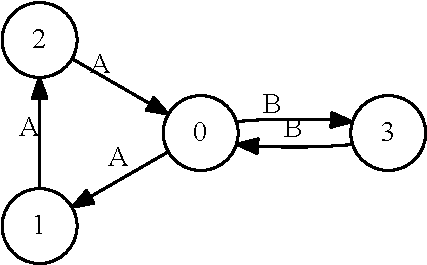
\includegraphics[width=\textwidth]{dot/input.pdf}
        \caption{The map of School (input graph $M$)}
        \label{input}        
		\vspace{1cm}
	\end{subfigure}
	~	
	\begin{subfigure}[b]{0.45\textwidth}
   \[
\begin{array}{rl}
   0:& S \rightarrow a \ S \ b \\
   1:& S \rightarrow Middle \\
   2:& Middle \rightarrow a \ b
\end{array}
\]
   \caption{Grammar $G_1$ for language $L=\{a^n b^n; n \geq 1\}$ with additional marker for the middle of a path}
   \label{grammarG}        
	\end{subfigure}
    \end{center}
\caption{An example: input graph and grammar}
\label{exampleData}
\end{figure}


You want to find a path from your current position to the same floor in another tower. 
Map with all such paths can help you.
But orienteering is not your forte, so it would be great if the structure of the paths were as simple as possible and all paths had additional checkpoints to control your rout.

It is evident that the simplest structure of required paths is $\{ab, aabb, aaabbb, \dots\}$.
In terms of our definitions, it is necessary to find all paths $p$ such that $\Omega(p) \in \{a^n b^n, n \geq 1\}$ in the graph $M=(\{0;1;2;3\},E,\{a;b\})$ (figure~\ref{input}).

Unfortunately, language $\mathcal{L} = \{a^n b^n; n \geq 1\}$ is not regular which restricts the set of tools you can use. 
Another problem is the infinite size of solution, but, being incapable to comprehend an infinite set of paths, you want to get a finite map.  
Moreover, you want to know structure of paths in terms of checkpoints.

We are not aware of any existing tools which can solve this problem, thus we have created such tool.
Let us show how to get a map which helps to navigate in this strange School.

Fortunately, the language $\mathcal{L} = \{a^n b^n; n \geq 1\}$ is a context-free language and it can be specified with context-free grammar. 
The fact that one language can be described with multiple grammars allows to add checkpoints: additional nonterminals can mark required parts of sentences.
In our case, desired checkpoint can be in the middle of the path.
As a result, required language can be specified by the grammar $G_1$ presented in figure~\ref{grammarG}, where $N = \{s; \text{\textit{Middle}}\}$, $\Sigma = \{a; b\}$, and $S$ is a start nonterminal.

Now, let us show that SPPF can be a solution for this problem.
SPPF for data from example is presented in figure~\ref{SPPF}.
Each terminal node corresponds to the edge in the input graph: for each node with label $(v_0, T, v_1)$ there is $e\in E: e=(v_0,T,v_1)$.
Extensions stored in SPPF nodes allow us to check whether path from $u$ to $v$ exists and to extract it by SPPF traverse. 

\begin{figure*}[ht]
    \begin{center}
    \centering
    \begin{subfigure}[b]{0.3\textwidth}
         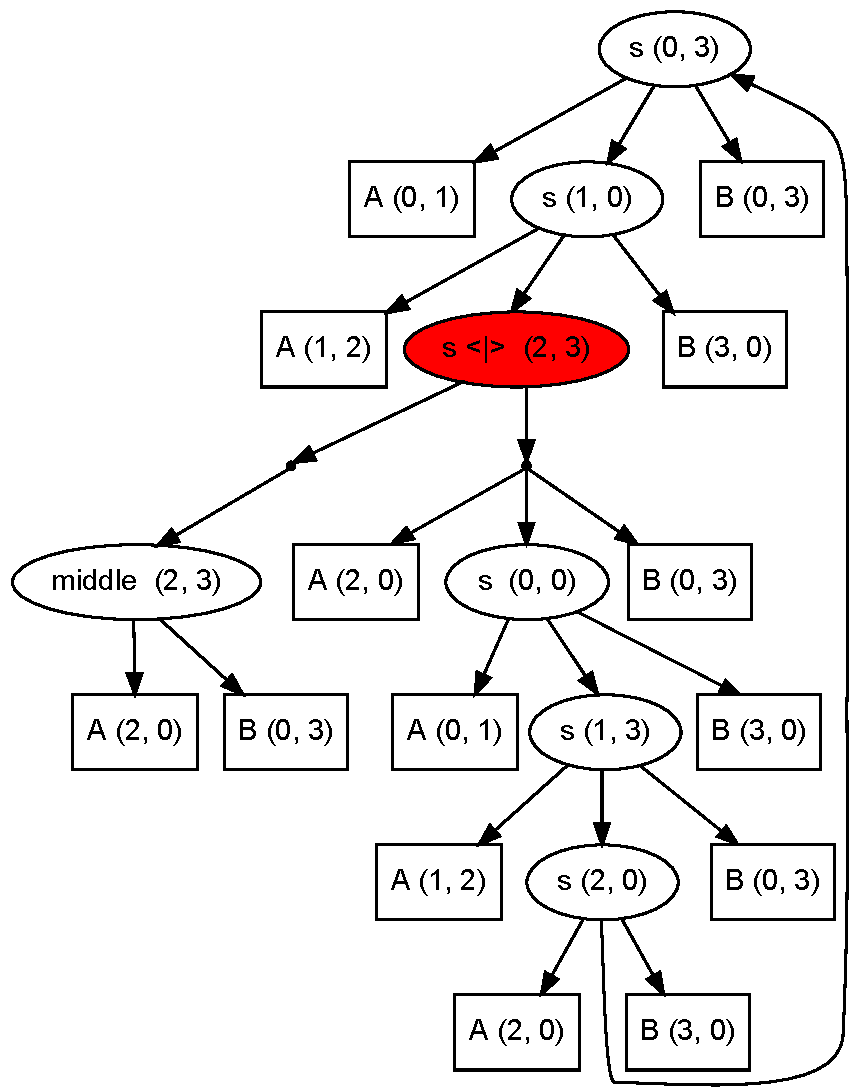
\includegraphics[width=\textwidth]{dot/AnBn.pdf}
        \caption{Result SPPF}
        \label{SPPF}        
    \end{subfigure}
    ~
    \begin{subfigure}[b]{0.3\textwidth}
        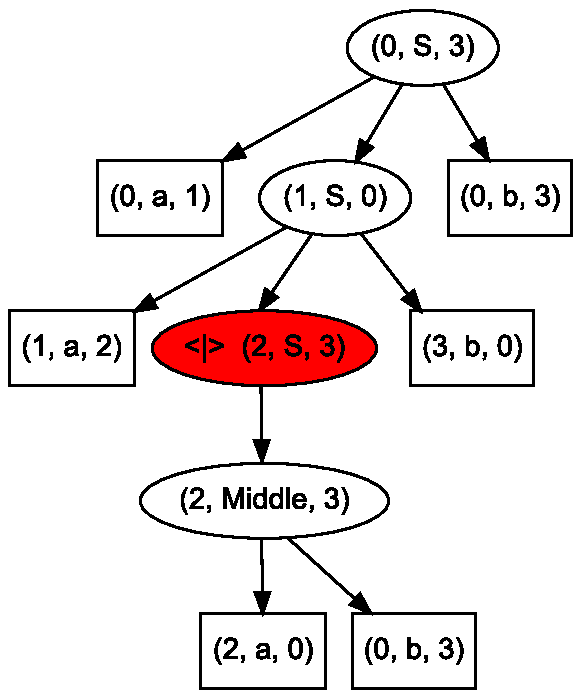
\includegraphics[width=\textwidth]{dot/AnBn_2.pdf}
        \caption{Derivation tree for $p_0$}
        \label{tree1}        
    \end{subfigure}
    ~
    \begin{subfigure}[b]{0.3\textwidth}
        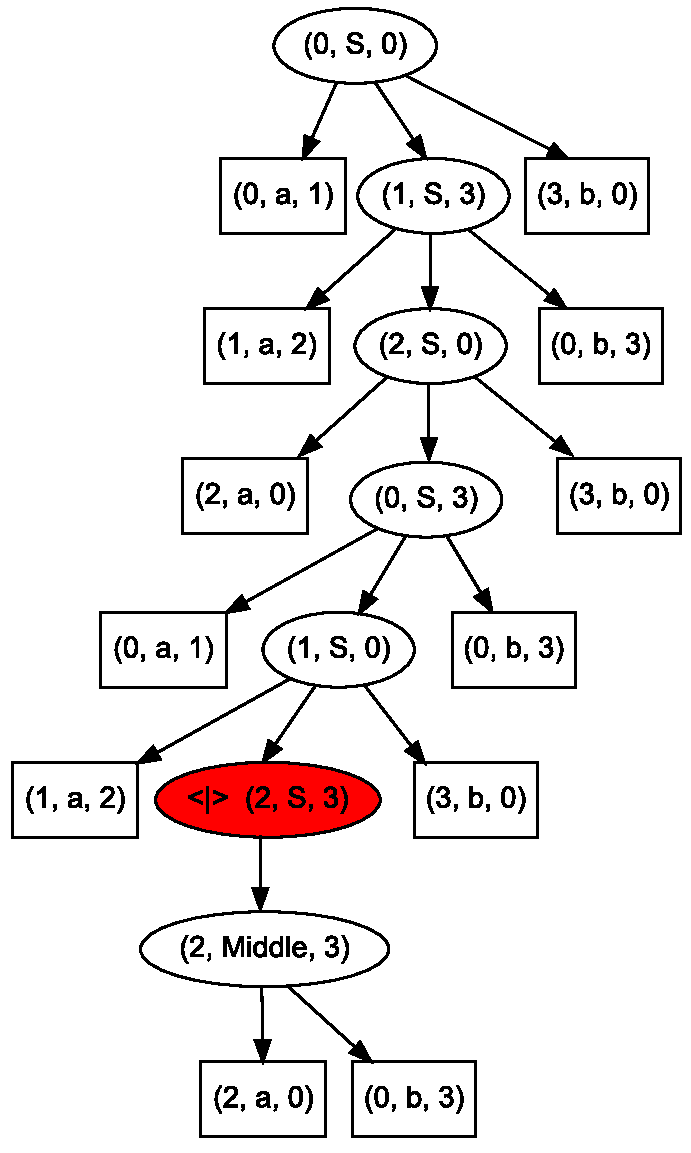
\includegraphics[width=\textwidth]{dot/AnBn_1.pdf}
        \caption{Derivation tree  for $p_1$}
        \label{tree2}        
    \end{subfigure}
    \caption{SPPF and examples of trees for specific paths for data from example (fig~\ref{exampleData}). Presented version does not contains redundant nodes, and we duplicate terminal nodes only for figure simplification.
    We use filled shape and label of form $(<\mkern-11mu | \mkern-11mu> (i, N, j))$ for nonterminal node to denote that there are multiple derivations from nonterminal $N$ for substring $\omega[i..j-1]$.	
	%\\
	%$p_0=\{(0,a,1);(1,a,2);(2,a,0);(0,b,3);(3,b,0);(0,b,3)\}$  \\
    %$p_1=\{(0,a,1);(1,a,2);(2,a,0);(0,a,1);(1,a,2);(2,a,0);(0,b,3);(3,b,0);(0,b,3);\\(3,b,0);(0,b,3);(3,b,0)\}.$
}
    \label{sppfSample}
    \end{center}                
\end{figure*}

As an example of derivation structure usage, we can find a middle of any path in example simply by finding correspondent nonterminal \textit{Middle} in SPPF.
So we can find out that there is only one (common) middle for all results, and it is a vertex with $id = 0$.

Lets find paths $p_i$ such that $S {\xRightarrow[G_1]{}}^{*} \Omega(p_i)$ and $p_i$ starts from the vertex $0$.
To do this, we should find vertices with label $(0, S, \_)$ in SPPF.
(There are two vertices with such labels: $(0, S, 0)$ and $(0, S, 3)$.)
Then let us to extract corresponded paths from SPPF.
There is a cycle in SPPF in our example, so there are \textbf{at least} two different paths: $p_0=\{(0,a,1);(1,a,2);(2,a,0);(0,b,3);(3,b,0);(0,b,3)\}$ and 
$
p_1=\{(0,a,1);(1,a,2);(2,a,0);(0,a,1);(1,a,2);(2,a,0);(0,b,3);(3,b,0);(0,b,3);\\(3,b,0);(0,b,3);(3,b,0)\}.
$ Trees for these paths are presented in figures~\ref{tree1} and~\ref{tree2} respectively.
%\end{align*}

We demonstrate that SPPF which was constructed by described algorithm can be useful for query result investigation. 
But in some cases explicit representation of matched subgraph is preferable, and required subgraph may be extracted from SPPF trivially by its traversal.


\section{Algorithm For Graph Parsing}
We propose a context-free language constrained path problem solution which allows to find all paths in graph. Paths are satisfied specified arbitrary context-free grammar. The algorithm constructs implicit representation of result. The results are represented with parsing forest of all possible parsing trees. 
Finite representation of result set with structure related to specified grammar may be useful not only for results understanding and processing but also for query debugging especially for complex queries. 

Our solution is based on generalized LL (GLL)~\cite{scott2010gll, FastPracticalGLL} parsing algorithm which allows to process ambiguous context-free grammars.
%Complexity is $O(n^3)$ in worst case and linear for unambiguous grammars, that better than complexity of CYK and Earley which used as base in other solutions (for example~\cite{ConjCFPathQuery}, ~\cite{GraphQueryWithEarley}).
%This fact allow to demonstarte better performance on linear subgraphs and unambiguous grammars.
%Also it is not necessary to transform input grammar to CNF which required for CYK which allow to avoid grmmar size decreasing.
%It is important because real performance of parsing algorithm is sensetive to grammar size.


\subsection{Generalized LL Parsing Algorithm}

Generalized LL (GLL) is generalized top-down parsing algorithm which handle all context-free grammars (including left recursive) with worst-case cubic time complexity and linear for LL grammars.
GLL is native for grammar, can be simple created !!!!!!! and debugging. Generalised algorithms look through all possible derivation in grammar for input. If current parsing branch is wrong the analisys (!??) process cotinious with others. 
GLL uses descriptors mechanism to store all parsing branches. Descriptors are four (!!???!!) elements which fully (??!!!) describes current parser state. Descriptor is a quadriple $(L, s, j, a)$ where $L$ is a line label, $s$ is a stack node, $j$ is a position in the input, and $a$ is a node of derivation tree. GLL parsers, like recursive descent parsers, consist of functions for every nonterminal and one dispatching function. Every function has label and a function gets control from another function due the call by the name. Process of analisys consist of calling function and tarts from the function for start nonterminal. !!!!!!!!!!!!!!!  нужно перейти от того, что лэйблы в оригинале и у нас!!!!!!!!!
Stack in parsing process is used to store return information for the parser -- a name of function which would be called when current function will stop work. As previously mentioned, generalised parsers process all possible derivation branches. For every branch parser must store it's own stack. It leads to OOM. !!!!  
Graph structured stack (GSS)~\cite{Tomita} is used to solve this problem. GSS allows to combine stacks to prevent duplication. Stacks with common part are combined to one graph structure and it stores only one node for evey analysis branch except whole stack. It allows to reduce (требуюмую) memory significantly. 
In GLL each GSS node contains pair -- position in input and grammmar slot. Grammar slot is like LR-slot. Slot is a grammar rule and position in it (for example !!!!).

The next part of the descriptor is a tree node. Parsers build derivation tree using input and grammar. There are more than one tree for ambigious grammar and generalised algorithms builds all derivation trees. Special data structure -- SPPF -- is used to reduce space required for tree storage.

\subsection{Shared packed parse forest}

Shared Packed Parse Forest (SPPF)~\cite{SPPF} is a spetial data structure for derivation forest compact representation which allow to reuse common nodes and subtrees.
As a result multiple derivation trees, which can be produced in case of ambiguos grammar, can be compressed in one SPPF with optimal reusing of common parts.  
Binarized form of SPPF proposed in~\cite{brnglr} and it allow to achive worst-case cubic space complexity.
GLL can use SPPF~\cite{gllParsingTree} for results representation achive cubic space complexity with binarised version.

Let we present an example of SPPF for ambiguos grammar $G_0$ (pic~\ref{grammarG0}).

\begin{figure}[h]
   \begin{center}
\begin{verbatim}
   0: s = NUM
   1: s = LBR s RBR
   2: s = s s
\end{verbatim}
   \caption{Grammar $G_0$}
   \label{grammarG0}        
   \end{center}
\end{figure}

Here \verb|N| is token for number, \verb|L| and \verb|R| are tokens for '(' and ')'  respectively.

Let we parse the sentence \verb|"()()()"|. 
There are two diferent lefmost derivations of this sentence in grammar $G_0$ ($\rightarrow ^ n$ denote an application of production with nimber $n$): 
\begin{enumerate} 
    \item $s \rightarrow ^ 2 s s \rightarrow ^ 2 s s s \rightarrow ^ 1 L s R s s \rightarrow ^ 0 L N R s s \rightarrow ^ 1 
    L N R L s R s \rightarrow ^ 1 L N R L s R s \rightarrow ^ 0 L N R L N R s \rightarrow ^ 1 L N R L N R L s R \rightarrow ^ 0 L N R L N R L N R$
    \item $s \rightarrow ^ 2 s s \rightarrow ^ 1 L s R s  \rightarrow ^ 0 L N R s \rightarrow ^ 2 L N R s s  \rightarrow ^ 1 
    L N R L s R s \rightarrow ^ 1 L N R L s R s \rightarrow ^ 0 L N R L N R s \rightarrow ^ 1 L N R L N R L s R \rightarrow ^ 0 L N R L N R L N R$
\end{enumerate}
 
    As far as there are tho different derivations, SPPF should contains two different trees and it is presented in figure~\ref{sppfSample}: result SPPF(fig. ~\ref{sppf}) and trees for derivation 1(fig.~\ref{tree1}) and derivation 2(fig.~\ref{tree2}) respectively. 
 
\begin{figure*}[ht]
    \begin{center}
    \centering
    \begin{subfigure}[b]{0.3\textwidth}
        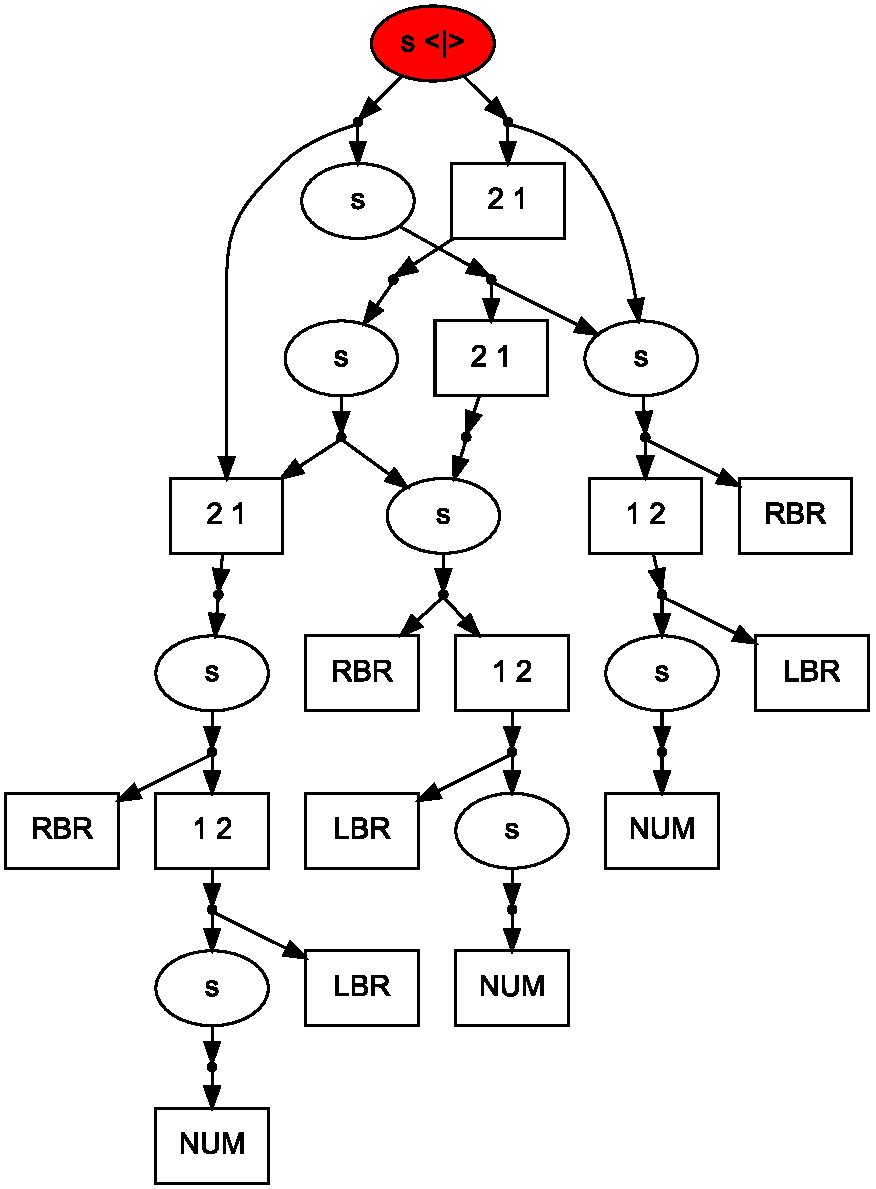
\includegraphics[width=\textwidth]{dot/Brackets.pdf}
        \caption{SPPF}
        \label{sppf}        
    \end{subfigure}
    ~
    \begin{subfigure}[b]{0.3\textwidth}
        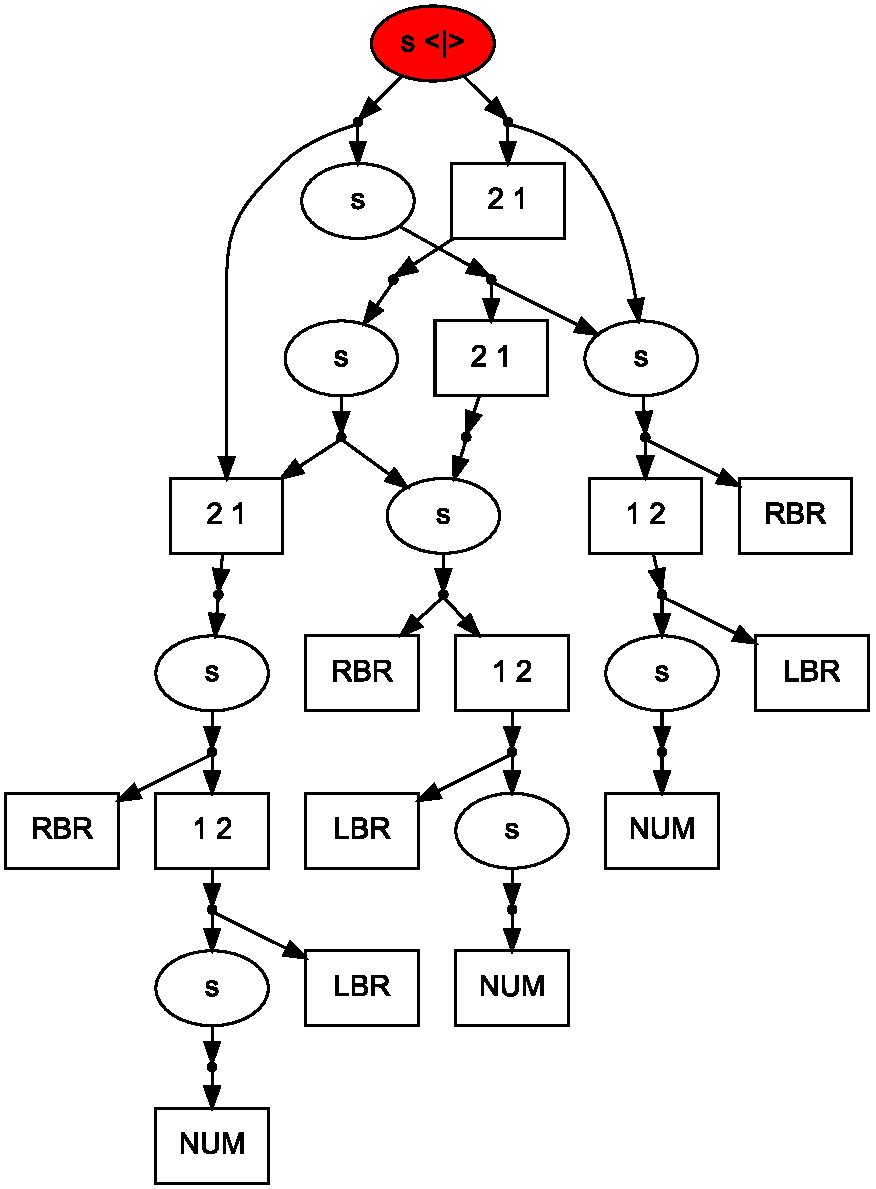
\includegraphics[width=\textwidth]{dot/Brackets.pdf}
        \caption{Tree for derivation 1}
        \label{tree1}        
    \end{subfigure}
    ~
    \begin{subfigure}[b]{0.3\textwidth}
        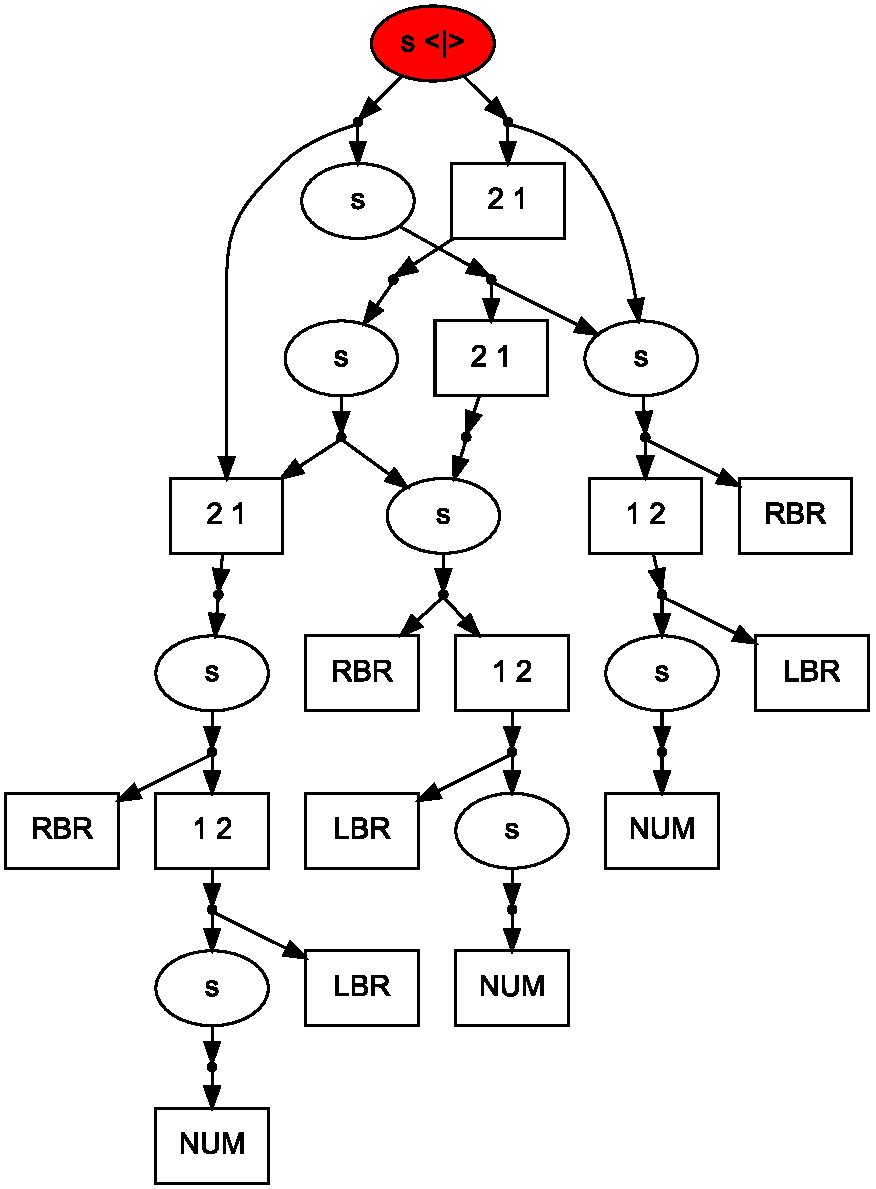
\includegraphics[width=\textwidth]{dot/Brackets.pdf}
        \caption{Tree for derivation 2}
        \label{tree2}        
    \end{subfigure}
    \caption{SPPF for sentence \textbf{\texttt{"(1)(2)(3)"}} and grammar $G_0$}
    \label{sppfSample}
    \end{center}                
\end{figure*}

Binarised SPPF can be represented as a graph where each node has one of four types: 

\begin{itemize}
    \item terminal node with label $(i,T,j)$;
    \item nonterminal node with label $(i,N,j)$;
    \item intermidiate node with label $(t,i,j)$ where $t$ is a grammar slot;
    \item packed node with label $(N : \gamma \cdot, k)$;
\end{itemize}
, and one of nodes can be marked as 'root' --- node for start nonterminal.

Further in our examples we will remove redudant intermidiate and packed nodes from SPPF to simplify it and decrease size of structure.

\subsection{GLL-based graph parsing}
(!!!!!Нужен какой-то переход или рассказ про то, как мы в виде графа представляем вход!!!!!!11)
In order to adapt GLL for graph parsing we need only use graph verticea as position in input.
As far as we work with context-free languages it is not important how this descriptor was created, and so descriptors management and other basic mechanisms of original algorithm can be reused ``as is''. 
We can merge it if they are equal. (!!!!!!!ВОТ эти два предожения вообще не нужны, кажется, но надо подумать!!!!!!!!!!!!!!) 

We implement some optimizations:~\cite{FastPracticalGLL}

We also use binarised SPPF for result representation whish allow to simplify query debugging and result explortion. (!!!!!!А что это  зачем?!!!!!!!)
In our case more then one root may be specified. For example, look at picture!!!! 
We 

$\mathbb{P}:G, M, StartVset, FinalVSet \rightarrow SPPF$
In details, main function input is graph $M$, set of start vertices $V_s\subseteq V$, set of final vertices $V_f\subseteq V$, grammar $G_1$.
Output is Shared Packed Parse Forest (SPPF)~\cite{SPPF} --- finite data structure which contains all derivation trees for all paths in $M$, $\Omega(p) \in L(G_1)$ and allows to reconstruct any of paths implicitly.
As far as we can specify sets of start and final vertices, our solution can find all paths in graph, all paths from specified vertex, all paths between specified vertices. 
Also SPPF represents a structure of paths in terms of derivation which allow to get more useful 
information about result. 
Binarized SPPF is at most cubic in terms of result size. 
Any path can be extracted in the linear time.


\subsection{Complexity}

Time complexity estimation in terms of input graph and grammar size is pretty similar to estimation of GLL complexity provided in~\cite{gllParsingTree}.

\begin{lemma}\label{lem:Descriptors}
For any descriptor $(L,u,i,w)$ either $w = \$$ or $w$ has extension $(j,i)$ where u has index $j$.
\end{lemma}
\begin{proof}
Proof of this lemma is the same as provided for original GLL in~\cite{gllParsingTree} because main function used for descriptors creation was not changed.
\end{proof}


\begin{mytheorem}\label{thm:GSSSpace}
The GSS generated by GLL-based graph parsing algorithm for grammar $G$ on input graph $M=(V,E,L)$ has at most $O(|V|)$ vertices and $O(|V|^2)$ edges.
\end{mytheorem}

\begin{proof}

Proof is the same as the proof of \textbf{Theorem 2} from~\cite{gllParsingTree} because structure of GSS was not changed. 

\end{proof}

\begin{mytheorem}\label{thm:SPPFSpace}
The SPPF generated by GLL-based graph parsing algorithm on input graph $M=(V,E,L)$ has at most $O(|V|^3 + |E|)$ vertices and edges.
\end{mytheorem}

\begin{proof}
Let us estimate the number of nodes of each type.
\begin{itemize}
\item \textbf{Terminal nodes.} 
Each of them is labeled with $(T, v_0, v_1)$, and such label can be created only if there is such $e \in E$ that $e=(v_0,T,v_1)$. 
Note, that there are no duplicate edges. 
Hence there are at most $|E|$ terminal nodes.
\item \textbf{$\varepsilon$ nodes} are labeled with $(\varepsilon, v ,v)$, hence there are at most $|V|$ of them. 
\item \textbf{Nonterminal nodes} have labels of form $(N,v_0,v_1)$, so there are at most $O(|V|^2)$ of them.
\item \textbf{Indeterminate nodes} have labels of form $(t,v_0,v_1)$, where $t$ is grammar slot, so there are at most $O(|V|^2)$ of them.
\item \textbf{Packed nodes} are children of intermediate or nonterminal nodes and have label of form $(t,v)$ where $t$ is a grammar slot $N \rightarrow \alpha \cdot \beta$.
There are at most $O(|V|^2)$ parents for packed nodes and each of them can have at most $O(|V|)$ children.
\end{itemize}

As a result there are at most $O(|V|^3 + |E|)$ nodes in SPPF.

The packed nodes have at most two children so there are at most $O(|V|^3 + |E|)$ edges with source in packed node. 
Nonterminal and intermediate nodes have at most $O(|V|)$ children and all of them are packed nodes.
Thus there are at most $O(|V|^3)$ edges with source in nonterminal or intermediate nodes. As a result there are at most $O(|V|^3 + |E|)$ edges in SPPF.


\end{proof}

\begin{mytheorem}
The space complexity of GLL-based graph parsing algorithm for graph $M=(V,E,L)$ is at most $O(|V|^3 + |E|)$.
\end{mytheorem}

\begin{proof}

From theorems~\ref{thm:GSSSpace} and~\ref{thm:SPPFSpace} we have that space required for main data structures is at most $O(|V|^3 + |E|)$. 

\end{proof}


\begin{mytheorem}\label{thm:complexity}
The runtime complexity of GLL-based graph parsing algorithm for graph $M=(V,E,L)$ is at most $$O\left(|V|^3*\max\limits_{v \in V}\left(deg^+\left(v\right)\right)\right).$$
\end{mytheorem}

\begin{proof}

From Lemma~\ref{lem:Descriptors} we get that there are at most $O(|V|^2)$ descriptors. 
Complexity of all functions are the same as in proof of \textbf{Theorem 4} from~\cite{gllParsingTree} except \textbf{Processing} function where we should process not single next input token, but the whole set of outgoing edges.
Thus, for each descriptor we should examine at most $$\max\limits_{v \in V}\left(deg^+\left(v\right)\right)$$ edges where $deg^+(v)$ is outdegree of vertex $v$.

Thus, worst-case complexity of proposed algorithm is $$O\left(V^3*\max\limits_{v \in V}\left(deg^+\left(v\right)\right)\right).$$
\end{proof}

%Also we can get averege-case complexity by calculate averege outdegree:
%\begin{align} \label{eq:avg}
%  & O\left(|V|^3*\frac {\sum\limits_{v \in V} deg^+(v)}{|V|}\right) = \nonumber \\
%  & O\left(|V|^2*\sum\limits_{v \in V} deg^+(v)\right) = \nonumber \\
%  & O\left(|V|^2*|E|\right) 
%\end{align}

From theorem~\ref{thm:complexity} we can get estimations for linear input and for LL grammars: $\text{for any } v \in V$ it is true, that $deg^+(v) \leq 1$, so $\max\limits_{v \in V}(deg^+(v))  = 1 $ and we get $O(|V|^3)$, as expected. 
For LL grammars and linear input complexity should be $O(|V|)$ for the same reason as for original GLL.
 

As discussed in~\cite{modellingGLL} achieving of theoretical complexity required special data structures which can be irrational for practice implementation and it is necessary to find balance between performance, software complexity, and hardware resources.
As a result in practice we can get slightly worse performance than theoretical estimation.

Note that result SPPF contains only paths matched specified query, so result SPPF size is $O(|V'|^3 + |E'|)$ where $M'=(V',E',L')$ is a subgraph of input graph $M$ which contains only matched paths.
Also note that each specific path can be explored with linear SPPF traversal. 

\subsection{Example}

Let us present a solution of task introduced in section~\ref{motivExample}: grammar $G_1$ is a query and we want to find all paths in graph $M$ (presented in picture~\ref{input}) matching this query.
Result SPPF for this input is presented in picture~\ref{SPPF}. Note that presented version does not contains obsolete nodes.
Each terminal node corresponds with edge in the input graph: for each node with label $(v_0, T, v_1)$ there is $e\in E: e=(v_0,T,v_1)$.
We duplicate terminal nodes only for figure simplification.

\begin{figure}[h]
    \begin{center}
        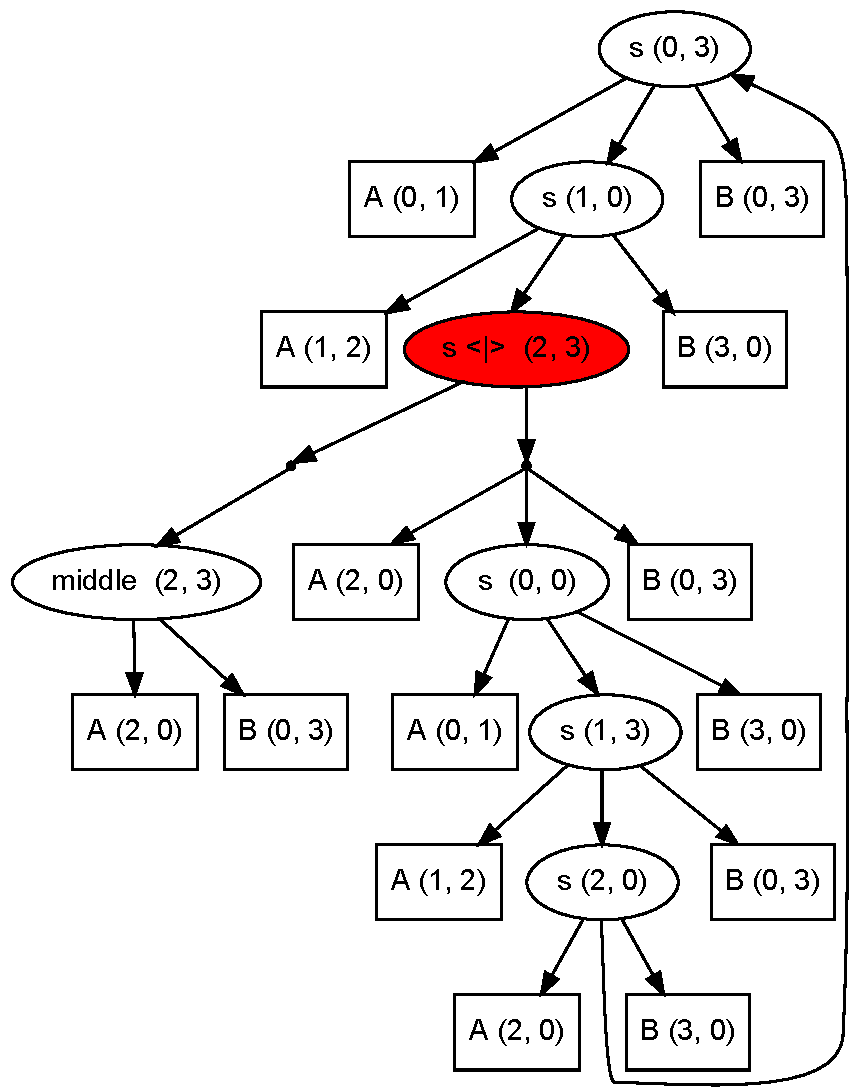
\includegraphics[width=8cm]{dot/AnBn.pdf}
        \caption{Result SPPF for input graph $M$(pic.~\ref{input}) and query $G_1$(pic.~\ref{grammarG})}
        \label{SPPF}        
    \end{center}
\end{figure}

    
As an example of derivation structure usage we can find 'middle' of any path in example above simply by finding correspondent nonterminal $middle$ in SPPF.
So we can find out that there is only one common ancestor for all results, and it is vertex with $id = 0$. 

Extensions stored in nodes allow us to check whether path from $u$ to $v$ exists, and to extract it. 
To extract specified path we need only traverse SPPF, and it can be done in linear time (in terms of SPPF size). 

Lets find paths satisfying specified in $G_1$ constraints from vertex $0$.
To do this we should find vertices with label $(0, s, \_)$ in SPPF.
We can see that there are two vertices with label matched this pattern: $(0, s, 0)$ and $(0, s, 3)$.
At the next step let us to extract corresponded paths from SPPF.
In our example there is cycle in SPPF so there are \textbf{at least} two different paths: $$p_0=\{(0,A,1);(1,A,2);(2,A,0);(0,B,3);(3,B,0);(0,B,3)\}$$ and 
\begin{align*}
p_1=\{&(0,A,1);(1,A,2);(2,A,0);(0,A,1);(1,A,2);(2,A,0);\\ &(0,B,3);(3,B,0);(0,B,3);(3,B,0);(0,B,3);(3,B,0)\}.
\end{align*}


Thus SPPF which was constructed by described algorithm can be useful for query result investigation. 
But in some cases explicit representation of matched subgraph is preferable, and required subgraph that may be extracted from SPPF trivially by its traversal.

In order to test the resulting solution we have implemented the frontend as a plugin using ReSharper SDK, so it can be installed into ReSharper, Rider and InspectCode.
The source code is parsed by internal ReSharper tools and the result is used to produce graphs and meta-information.
The issues found by the backend are shown using code highlighting.

The first analysis which has been implemented is the considered taint tracking analysis.
It is defined just by the PDA constructed in the section 2 translated into the code with some slight modifications which make it possible to process interactions with object fields.
To provide more information about an issue found by this analysis, the higlighting is accompanied by bulbs containing the full path of tainted variable from the source to the sink represented as the sequence of operations.

\subsection{Sample cases}

Let's look closer at properties of the resulting soluiton.
All these properties are illustrated by screenshots taken exactly from the runned Rider IDE with some small relocations of bulbs to make them not to overlap the code.

Firstly, the solution ensures flow sensitivity. I.e. it processes flow of variables passed into methods and returned from them correctly.
Which can be seen at fig~\ref{fig:ReturnsAndBrackets}.
This example illustrates the most common cases of interprocedural data passing.
\textit{Brackets} method gets the data, performs some computations on them and returns the result.
Invocations at lines 37 and 38 shows that the solution can distinguish two data flow paths despite both of them passes through the same method.
So, \textit{e} becomes tainted because \textit{c} is tainted and \textit{f} does not because \textit{d} is clear.
Moreover, the solution can track paths where passes and returns do not form the correct bracket sequence that is shown by method \textit{PostSource} which does not take any parameter and just returns tainted data.

\begin{figure}[h]
	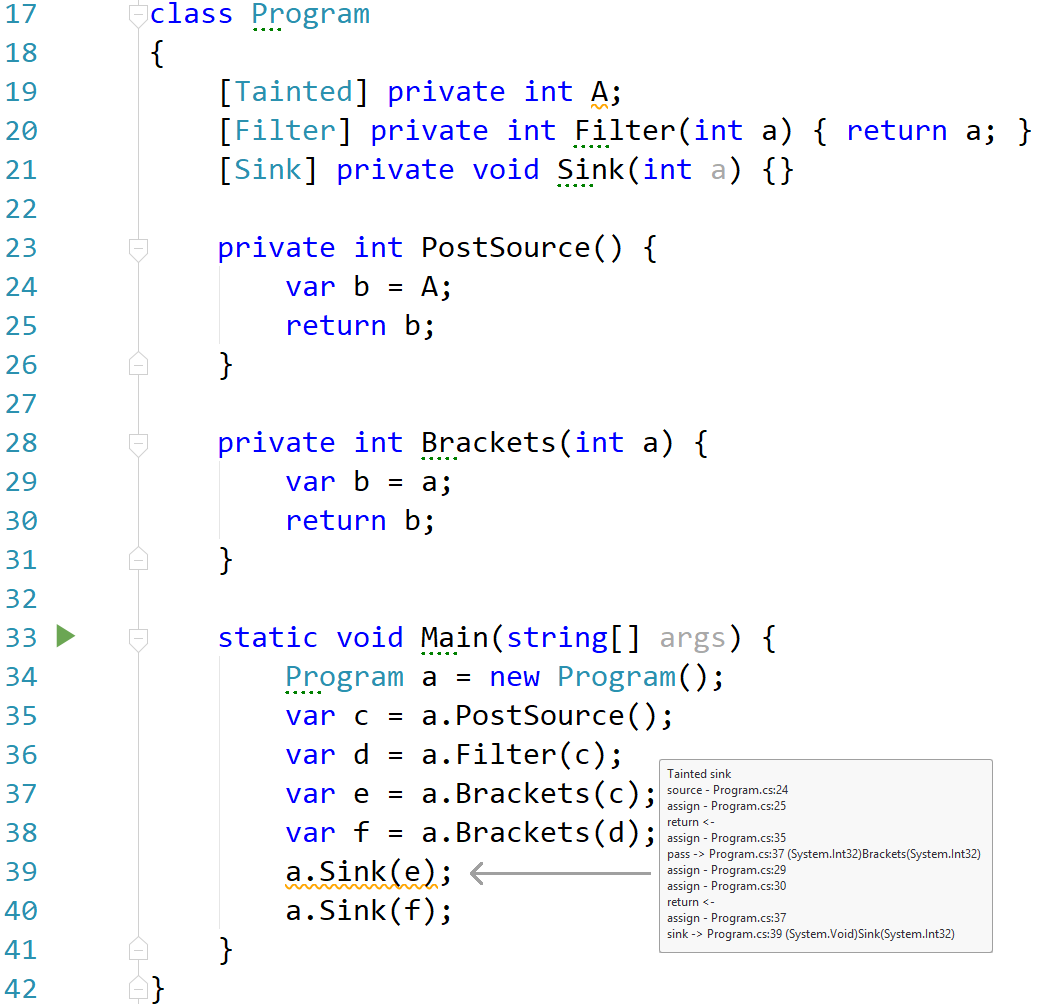
\includegraphics[width=\linewidth]{screenshots/ReturnsAndBrackets.png}
	\caption{Flow sensitivity}
	\label{fig:ReturnsAndBrackets}
\end{figure}

Secondly, the solution has the limited context sensitivity. I.e. it allows to track propagation of objects that are tainted by assigning of some fields inside them both by their own methods and by outer code interacting with their fields directly.
The first case is shown at fig~\ref{fig:ObjectTainting}.
There is the field \textit{B} at the line 18. 
This field can be used widely in the logic of the \textit{Container} class and by this the tainting of this field is considered as the tainting of the whole object.
However, while processing of the method \textit{Store} during the analysis it is hard to decide what the object need to be tainted because in the inner context of \textit{Store} it is just \textit{this} object.
I.e. we must consider the calling context to make such decision.
So, the solution provides this opportunity which is shown by lines 33-36 where the first invocation of \textit{Store} leads to the tainting of object \textit{d} and the second invocation does not taint object \textit{e}.

\begin{figure}[h]
	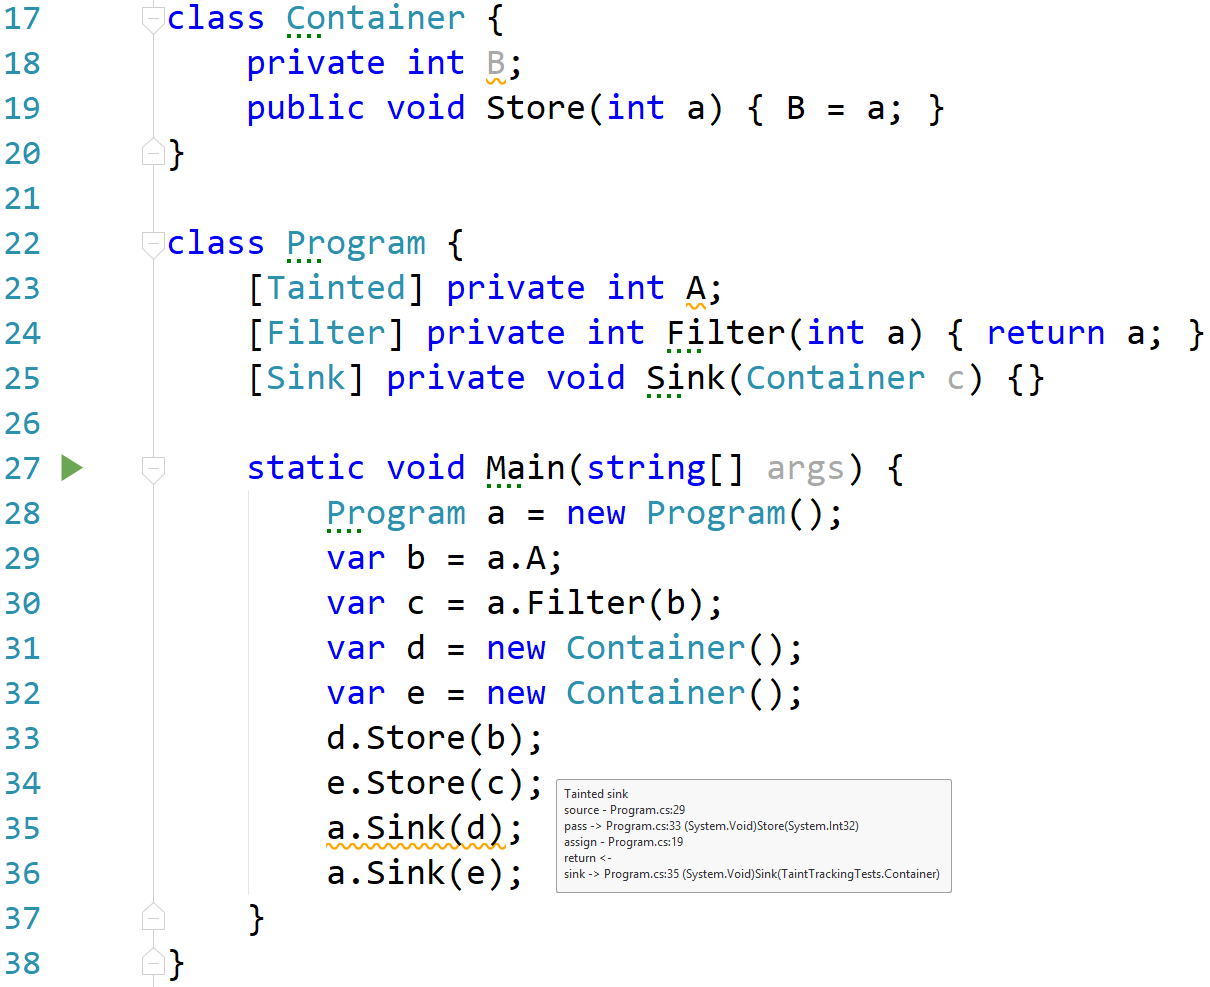
\includegraphics[width=\linewidth]{screenshots/ContextSensitivity.png}
	\caption{Tainting of an object by its own method}
	\label{fig:ObjectTainting}
\end{figure}

Finally, the solution works with any type of recursion and does not fall into infinite cycles.
It can be seen at fig.~\ref{fig:Recursion}.
This snippet contains two mutually recursive methods which pass the data to each other.
The solution checks all possible paths of passing even those which includes cyclic invocations and returns the passed variable to the point corresponding to the initial invocation.

\begin{figure}[h]
	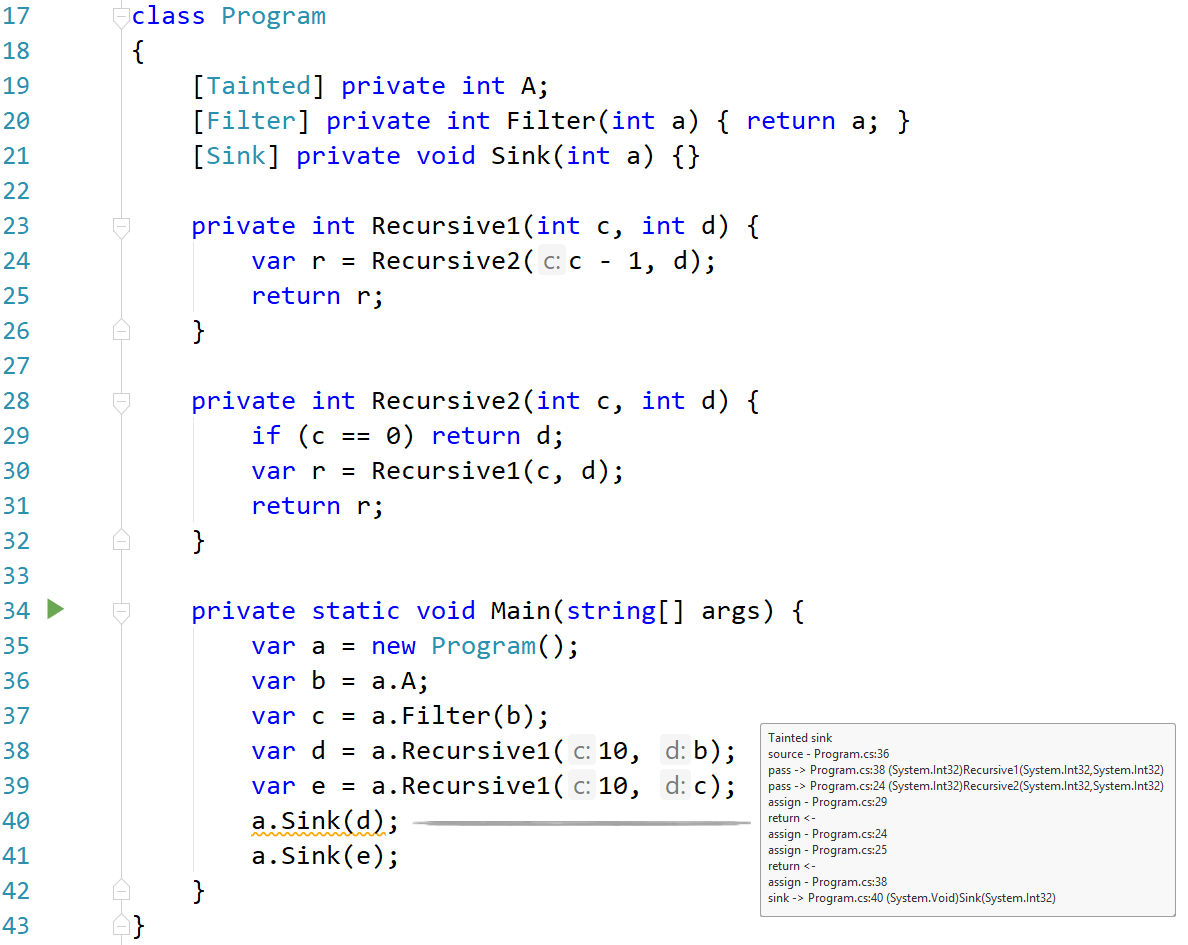
\includegraphics[width=\linewidth]{screenshots/Recursion.png}
	\caption{Recursive methods processing}
	\label{fig:Recursion}
\end{figure}

\subsection{Performance}

It is also necessary to measure the performance of the resulting solution.
Because the implemented taint tracking analysis forces to mark all participating entities manually, it is difficult to perform it on some large project.
However, there is another intermediate analysis which is runned before any other one to collect some information required by resolver.
In particular, it tracks propagation of all variables to discover all possible concrete types of each variable.
So, it involves each variable and each method in the whole program and thus the time and space required for execution of this analysis may be consistent estimation of the efficiency of the solution.

The code base that has been chosen as a source of data is the full solution of the Mono project.
(TODO: ADD SYSTEM CONFIGURATION).
The results is shown in the table~\ref{tab:Performance}.

\begin{table}[h]
	\begin{tabular}{|l|l|l|l|l|}
	\hline
		Project & Classes & Methods & \begin{tabular}[c]{@{}l@{}}Execution \\ time (s)\end{tabular} & \begin{tabular}[c]{@{}l@{}}Allocated \\ memory (GB)\end{tabular} \\ \hline
		Mono & 21013 & 192745 & $21\pm 0.5$ & $\sim 4.2$ \\ \hline
	\end{tabular}
	\caption{Performance}
	\label{tab:Performance}
\end{table}

\section{Conclusion}

We propose and implement in C\# programming language the generic framework for interprocedural static code analysis implementation.
This framework allows one to implement arbitrary interprocedural analysis in terms of CFL-reachability.
By using the proposed framework, we implement a plugin upon ReSharper infrastructure which provides simple taint analysis and demonstrate that our solution can handle important real-world cases.
Also we show that the proposed framework can be used for real-world solutions analysis.

One of the directions for future work is a creation of analysis and its evaluation on real-world projects.
By this way, we want to get information which helps to improve the usability of our framework: tune performance, improve API, etc.
Also we should improve documentation and create more examples of usage.

Another direction is a practical evaluation of automatic fix location prediction by using minimum cuts method~\cite{10.1007/978-3-319-63390-9_27}.

Also we want to compare the proposed approach with other generic CFL-reachability based approaches for interprocedural code analysis cretion. For example, fith generation-based approach~\cite{LPAR-21:Cauliflower_Solver_Generator_for}, which idea is similar to parser generators.


\bibliographystyle{abbrv}
\bibliography{ContextFreeConstrainedPathFindingInGraph}

\end{document}
